\documentclass{standalone}
\usepackage{tikz}
\usetikzlibrary{
  arrows,
  calc,
  decorations.pathmorphing,
  decorations.pathreplacing,
  decorations.markings,
  fadings,
  positioning,
  shapes,
  arrows.meta
}
\pgfdeclareradialshading{glow}{\pgfpoint{0cm}{0cm}}{
  color(0mm)=(white);
  color(5mm)=(white);
  color(9mm)=(black);
  color(10mm)=(black)
}

\begin{tikzfadingfrompicture}[name=glow fading]
  \shade [shading=glow] (0,0) circle (1);
\end{tikzfadingfrompicture}

\ifpdf
% Ensure reproducible output
\pdfinfoomitdate=1
\pdfsuppressptexinfo=-1
\pdftrailerid{}
\fi

\begin{document}

\begin{tikzpicture}
  % f_raman0 = 770.200516(24) MHz
  % f_pa0 = 288711.696(73) GHz
  % offset = 2.194(17) kHz/mW
  % strength = 4.1083(46) MHz GHz/mW
  \node at (-0.1, 0) {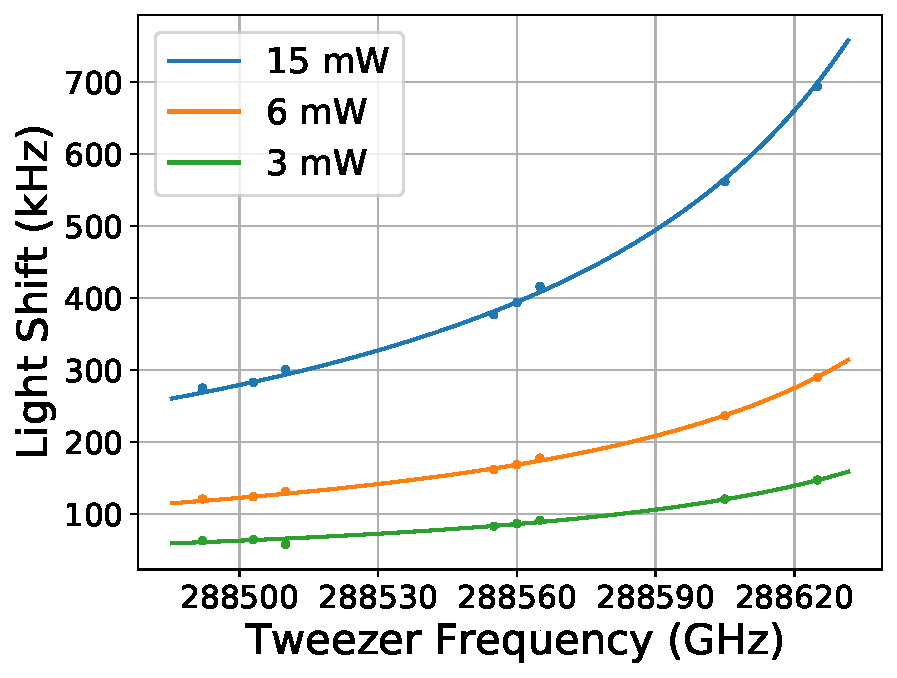
\includegraphics[height=3.9cm]{imgs/light_shift_fs.pdf}};
  \node at (1.58, 1.6) {\footnotesize (\textbf{a})};
  \node at (-0.65, 0.8) {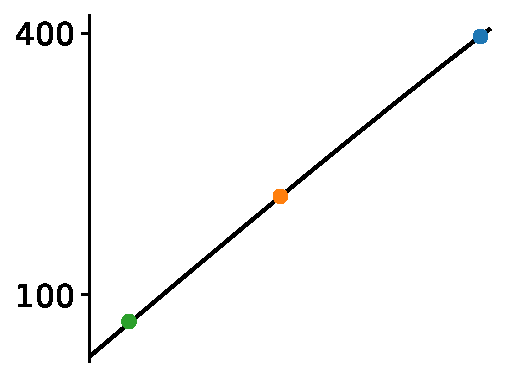
\includegraphics[height=2.13cm]{imgs/light_shift_560.pdf}};
  % offset = -2pi 68.0(53) Hz/mW^-1.29
  % strength = 2pi 25.79(60) kHz GHz/mW^-1.29
  \node at (5, 0) {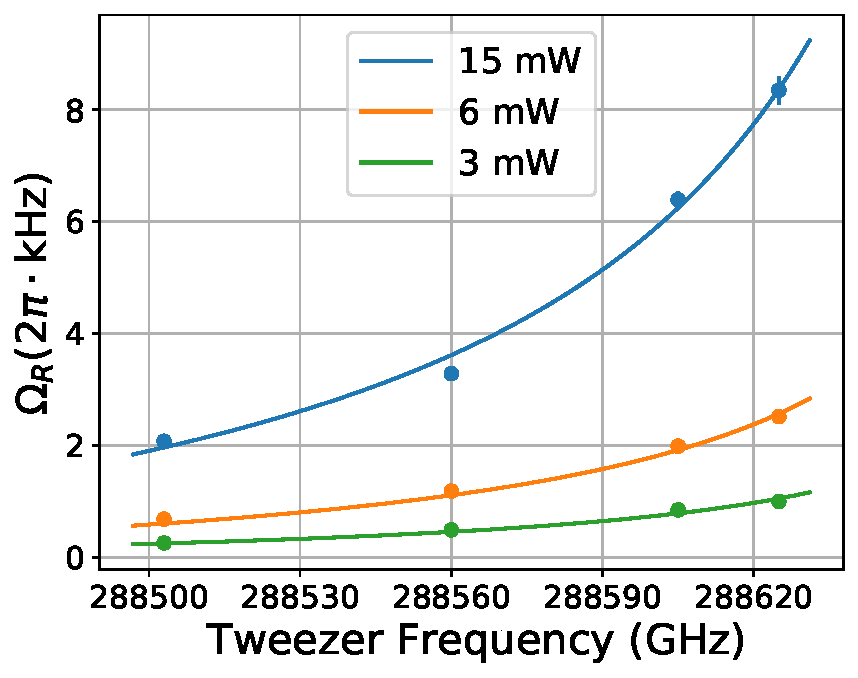
\includegraphics[height=3.9cm]{imgs/rabi_scaling.pdf}};
  \node at (6.7, 1.6) {\footnotesize (\textbf{b})};
  \node at (4.3, 0.68) {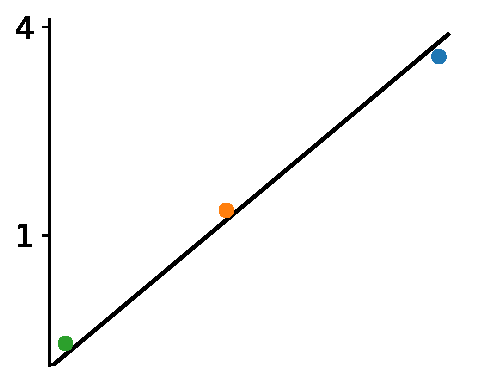
\includegraphics[height=2.4cm]{imgs/rabi_scaling_560.pdf}};
\end{tikzpicture}

\end{document}
